% !TEX TS-program = XeLaTeX
% use the following command: 
% all document files must be coded in UTF-8
\documentclass{textolivre}
% for anonymous submission
%\documentclass[anonymous]{textolivre}
% to create HTML use 
%\documentclass{textolivre-html}
% See more information on the repository: https://github.com/leolca/textolivre

% Metadata
\begin{filecontents*}[overwrite]{article.xmpdata}
    \Title{Aplicativos móveis como recursos didáticos digitais: um mapeamento na educação formal}
    \Author{Kadhiny Policarpo and Juliana Cristina Faggion Bergmann}
    \Language{pt-BR}
    \Keywords{telefone móvel \sep aplicativo móvel \sep recurso didático digital \sep língua estrangeira \sep educação formal}
    \Journaltitle{Texto Livre}
    \Journalnumber{1983-3652}
    \Volume{14}
    \Issue{3}
    \Firstpage{1}
    \Lastpage{14}
    \Doi{10.35699/1983-3652.2021.24923}

    \setRGBcolorprofile{sRGB_IEC61966-2-1_black_scaled.icc}
            {sRGB_IEC61966-2-1_black_scaled}
            {sRGB IEC61966 v2.1 with black scaling}
            {http://www.color.org}
\end{filecontents*}

% used to create dummy text for the template file
\definecolor{dark-gray}{gray}{0.35} % color used to display dummy texts
\usepackage{lipsum}
\SetLipsumParListSurrounders{\colorlet{oldcolor}{.}\color{dark-gray}}{\color{oldcolor}}

% used here only to provide the XeLaTeX and BibTeX logos
\usepackage{hologo}

% used in this example to provide source code environment
%\crefname{lstlisting}{lista}{listas}
%\Crefname{lstlisting}{Lista}{Listas}
%\usepackage{listings}
%\renewcommand\lstlistingname{Lista}
%\lstset{language=bash,
        breaklines=true,
        basicstyle=\linespread{1}\small\ttfamily,
        numbers=none,xleftmargin=0.5cm,
        frame=none,
        framexleftmargin=0.5em,
        framexrightmargin=0.5em,
        showstringspaces=false,
        upquote=true,
        commentstyle=\color{gray},
        literate=%
           {á}{{\'a}}1 {é}{{\'e}}1 {í}{{\'i}}1 {ó}{{\'o}}1 {ú}{{\'u}}1 
           {à}{{\`a}}1 {è}{{\`e}}1 {ì}{{\`i}}1 {ò}{{\`o}}1 {ù}{{\`u}}1
           {ã}{{\~a}}1 {ẽ}{{\~e}}1 {ĩ}{{\~i}}1 {õ}{{\~o}}1 {ũ}{{\~u}}1
           {â}{{\^a}}1 {ê}{{\^e}}1 {î}{{\^i}}1 {ô}{{\^o}}1 {û}{{\^u}}1
           {ä}{{\"a}}1 {ë}{{\"e}}1 {ï}{{\"i}}1 {ö}{{\"o}}1 {ü}{{\"u}}1
           {Á}{{\'A}}1 {É}{{\'E}}1 {Í}{{\'I}}1 {Ó}{{\'O}}1 {Ú}{{\'U}}1
           {À}{{\`A}}1 {È}{{\`E}}1 {Ì}{{\`I}}1 {Ò}{{\`O}}1 {Ù}{{\`U}}1
           {Ã}{{\~A}}1 {Ẽ}{{\~E}}1 {Ũ}{{\~u}}1 {Õ}{{\~O}}1 {Ũ}{{\~U}}1
           {Â}{{\^A}}1 {Ê}{{\^E}}1 {Î}{{\^I}}1 {Ô}{{\^O}}1 {Û}{{\^U}}1
           {Ä}{{\"A}}1 {Ë}{{\"E}}1 {Ï}{{\"I}}1 {Ö}{{\"O}}1 {Ü}{{\"U}}1
           {ç}{{\c{c}}}1 {Ç}{{\c{C}}}1
}


\journalname{Texto Livre}
\thevolume{14}
\thenumber{3}
\theyear{2021}
\receiveddate{\DTMdisplaydate{2020}{8}{14}{-1}} % YYYY MM DD
\accepteddate{\DTMdisplaydate{2021}{4}{5}{-1}}
\publisheddate{\DTMdisplaydate{2021}{9}{2}{-1}}
% Corresponding author
\corrauthor{Kadhiny Policarpo}
% DOI
\articledoi{10.35699/1983-3652.2021.24923}
%\articleid{NNNN} % if the article ID is not the last 5 numbers of its DOI, provide it using \articleid{} commmand
% list of available sesscions in the journal: articles, dossier, reports, essays, reviews, interviews, editorial
\articlesessionname{articles}
% Abbreviated author list for the running footer
\runningauthor{Policarpo e Bergmann}
%\editorname{Anna Izabella M. Pereira}
\sectioneditorname{Daniervelin Pereira}
\layouteditorname{Anna Izabella M. Pereira}


\title{Aplicativos móveis como recursos didáticos digitais: 
um mapeamento na educação formal}
\othertitle{Mobile applications as digital pedagogical resources: a mapping through formal education}
% if there is a third language title, add here:
%\othertitle{Artikelvorlage zur Einreichung beim Texto Livre Journal}

\author[1]{Kadhiny Policarpo \orcid{0000-0002-2097-6647} \thanks{Email: \url{kadhinymendonca@gmail.com}}}
\author[2]{Juliana Cristina Faggion Bergmann \orcid{0000-0002-0535-5279} \thanks{Email: \url{juliana.bergmann@ufsc.br}}}


\affil[1]{Universidade Federal de Santa Catarina, Programa de pós-graduação em Educação, Florianópolis, Santa Catarina, Brasil.}
\affil[2]{Universidade Federal de Santa Catarina, Departamento de Metodologia de Ensino, Florianópolis, Santa Catarina, Brasil.}

\addbibresource{article.bib}
% use biber instead of bibtex
% $ biber tl-article-template

% set language of the article
\setdefaultlanguage{portuguese}
\setotherlanguage{english}

% for spanish, use:
%\setdefaultlanguage{spanish}
%\gappto\captionsspanish{\renewcommand{\tablename}{Tabla}} % use 'Tabla' instead of 'Cuadro'
%\AfterEndPreamble{\crefname{table}{tabla}{tablas}\Crefname{table}{Tabla}{Tablas}}

% for languages that use special fonts, you must provide the typeface that will be used
% \setotherlanguage{arabic}
% \newfontfamily\arabicfont[Script=Arabic]{Amiri}
% \newfontfamily\arabicfontsf[Script=Arabic]{Amiri}
% \newfontfamily\arabicfonttt[Script=Arabic]{Amiri}
%
% in the article, to add arabic text use: \textlang{arabic}{ ... }

% to use emoticons in your manuscript
% https://stackoverflow.com/questions/190145/how-to-insert-emoticons-in-latex/57076064
% using font Symbola, which has full support
% the font may be downloaded at:
% https://dn-works.com/ufas/
% add to preamble:
% \newfontfamily\Symbola{Symbola}
% in the text use:
% {\Symbola }

% reference itens in a descriptive list using their labels instead of numbers
% insert the code below in the preambule:
\makeatletter
\let\orgdescriptionlabel\descriptionlabel
\renewcommand*{\descriptionlabel}[1]{%
  \let\orglabel\label
  \let\label\@gobble
  \phantomsection
  \edef\@currentlabel{#1\unskip}%
  \let\label\orglabel
  \orgdescriptionlabel{#1}%
}
\makeatother
%
% in your document, use as illustraded here:
%\begin{description}
%  \item[first\label{itm1}] this is only an example;
%  % ...  add more items
%\end{description}
 

% custom epigraph - BEGIN 
%%% https://tex.stackexchange.com/questions/193178/specific-epigraph-style
\usepackage{epigraph}
\renewcommand\textflush{flushright}
\makeatletter
\newlength\epitextskip
\pretocmd{\@epitext}{\em}{}{}
\apptocmd{\@epitext}{\em}{}{}
\patchcmd{\epigraph}{\@epitext{#1}\\}{\@epitext{#1}\\[\epitextskip]}{}{}
\makeatother
\setlength\epigraphrule{0pt}
\setlength\epitextskip{0.5ex}
\setlength\epigraphwidth{.7\textwidth}
% custom epigraph - END


% if you use multirows in a table, include the multirow package
\usepackage{multirow}

% add line numbers for submission
%\usepackage{lineno}
%\linenumbers

\begin{document}
\maketitle

\begin{polyabstract}
\begin{abstract}
O telefone móvel, mais precisamente o \emph{smartphone}, vem se destacando muito nos últimos anos muito por conta de sua mobilidade, por ser uma tecnologia nômade e também por ser metamídia, ou seja, convergem muitos meios de comunicação em um só aparelho \cite{suarez2019}. Dentro desse dispositivo, instalamos \textit{softwares}, chamados de aplicativos, que funcionam como atalhos para as atividades que queremos desempenhar \cite{gardner2014}, e que vão desde a comunicação até a locomoção, entre muitos outros. Entretanto, essa realidade é percebida de maneira efetiva dentro da escola e com objetivos pedagógicos. Sendo assim, esta revisão sistemática tem como intuito mapear, e conhecer o estado da arte, quanto ao uso de aplicativos móveis como recursos didáticos digitais nas salas de aula de língua estrangeira na educação básica. 

\keywords{Telefone móvel \sep Aplicativo móvel \sep Recurso didático digital \sep Língua estrangeira \sep Educação formal}
\end{abstract}

\begin{english}
\begin{abstract}
The smartphone has been taking a highlight place nowadays because of its mobility, for being a nomadic technology, and also for being a metamedia, in other words, it converges a lot of medias in one single device \cite{suarez2019}. On this gadget, we can download softwares, called applications, that work as shortcuts \cite{gardner2014} to activities that we want to perform, which can be from communication to locomotion activities and others. However, this reality has been perceived inside the school and with pedagogical goals. Therefore, this systematic review has the aim to map, and to acquire knowledge about the mobile applications as pedagogical resource in foreign language classroom at school.

\keywords{Mobile phone \sep Mobile app \sep Digital teaching resource \sep Foreign language \sep Formal education}
\end{abstract}
\end{english}

% if there is another abstract, insert it here using the same scheme
\end{polyabstract}


\section{Introdução}\label{sec-intro}
Os \textit{smartphones} seguem ganhando cada vez mais espaço em nossas vidas e em nossas atividades cotidianas. Inúmeras ações que desempenhamos atualmente são feitas através, acompanhadas ou mediadas por esse dispositivo móvel e por softwares nele instalados, chamados de aplicativos. Esses aplicativos, ou \textit{Apps}, são como atalhos para inúmeras atividades que desempenhamos \cite{gardner2014}, e que estão sempre ao alcance de nossas mãos, além de muitas vezes atuarem como extensão da nossa própria memória.

Entretanto, por mais que essa influência tecnológica esteja presente em nossas vidas e na sociedade, parece que ela não é vista, ou é ignorada, quando adentramos os muros das escolas. Dentro do ambiente escolar, muitas vezes os alunos têm que deixar de lado essas tecnologias, utilizadas por eles fora da escola, dando a sensação de uma dissociação da realidade dentro e fora da escola, o que sabemos que não é verídico, causando muitas vezes frustrações e o sentimento de desconexão escola-realidade por parte dos alunos. Isso acontece porque ainda há resistência por parte de professores e profissionais da educação, que creem que os dispositivos móveis não podem ser incorporados nas aulas. Essa visão também pode ser reflexo da falta de formação digital inicial e continuada de professores, que não tiveram a oportunidade de conhecer e avaliar de forma crítica o uso de tecnologias digitais em aula. Por outro lado, há pesquisas e estudos que apontam que essas tecnologias podem sim trazer benefícios desde que os objetivos pedagógicos norteiem essa utilização \cite{bannell2016, gardner2014, karsenti2014, perezgomez2012, saccol2011, unesco}.
	
Sendo assim, o objetivo desta revisão sistemática é mapear teses, dissertações e artigos publicados em três idiomas – português, inglês e espanhol – que abordem a temática do uso de aplicativos móveis como recursos didáticos nas aulas de língua estrangeira na educação básica, permitindo conhecer um pouco sobre o atual cenário dessa prática pedagógica através das tecnologias digitais do século XXI. A razão das escolhas desses idiomas é fundamentada pelas línguas de domínio da pesquisadora, juntamente com a relevância dessas línguas referente a publicações na área.

\section{Procedimentos metodológicos}
Essa revisão utilizará como norteadores metodológicos os estudos de \textcite{rother2007}, nos quais destaca 07 passos a serem seguidos com a finalidade de responder a uma pergunta específica, são eles: definição da questão norteadora, instituir as bases de dados e palavras-chave, estabelecer os critérios de exclusão e inclusão, busca na base de dados, selecionar os trabalhos usando os critérios estabelecidos, analisar e avaliar criticamente os estudos, sintetizar as informações, conclusão e publicação dos dados. 

\subsection{Questões norteadoras}

Algumas questões norteadoras foram levantadas a partir do problema de pesquisa.

\begin{itemize}
\item Questão um (Q1): Existem estudos que envolvam o uso de aplicativos como recurso didático nas aulas de língua estrangeira?
\item Questão dois (Q2): Quais os níveis de escolaridade contemplados pela utilização dos aplicativos móveis como recurso didático?
\item Questão três (Q3): Quais os principais objetivos das pesquisas que reporta usos de aplicativos móveis em sala de aula de LE? 
\item Questão quatro (Q4): Qual o objetivo linguístico para a utilização do aplicativo?
\item Questão cinco (Q5): Quais Apps foram utilizados e quais os conteúdos abordados neles?
\end{itemize}

\subsection{Estratégia de busca: base de dados e palavras}
As bases de dados escolhidas para esta pesquisa foram o Google Acadêmico, a ERIC (\emph{Education Resources Information Center}), Periódicos da Capes, SCIELO, BNTD (Biblioteca Digital Brasileira de Teses e Dissertações) e Base de Teses e Dissertações da Capes. A justificativa para essas escolhas é a importância e o lugar de destaque que essas bases de dados ocupam dentro da temática da presente pesquisa e no país. 

Os termos utilizados na busca foram nos idiomas português, inglês e espanhol, para uma maior abrangência em busca do atual estado da arte. Cada base de dados tinha diferentes modos de refinamento de pesquisa, por meio de \textit{string}, \textit{tags} e restritores (\Cref{tab1} e \Cref{tab2}), que foram utilizados de maneira a sistematizar e refinar os resultados. Um desses restritores foi limitar a busca das palavras-chave ao título e ao resumo. O período desta pesquisa compreendeu os meses de março e abril de 2019, finalizando no dia 07 de maio de 2019. 

\begin{table}[htpb]
\caption{\emph{String} de busca no Google Scholar, ERIC}
\label{tab1}
\centering
\begin{tabular}{p{0.15\textwidth}p{0.75\textwidth}}
\toprule 
\arrayrulecolor[gray]{.7}
Português & "aplicativo móvel" AND "língua estrangeira" OR “segunda língua” AND "recurso didático" OR "material didático"
\\
\midrule
Espanhol & "aplicación móvil" AND "lengua extranjera" AND "recurso didáctico" OR "material didáctico"
\\
\midrule
Inglês & "mobile application" OR "app" AND "foreign language" AND "pedagogical resource"
\\ 
\arrayrulecolor{black}
\bottomrule
\end{tabular}
\source{Elaborado pela própria autora (2019)}
\centering
\end{table}

\begin{table}[htpb]
\caption{\textit{String} de busca nos Periódicos da CAPES, SCIELO, BNTD e Base de Teses e Dissertações CAPES}
\label{tab2}
\centering
\begin{tabular}{p{0.15\textwidth}p{0.75\textwidth}}
\toprule 
\arrayrulecolor[gray]{.7}
Português & (aplicativo móvel) AND (língua estrangeira) AND (recurso didático)
\\
\midrule
Espanhol & (aplicación móvil) AND (lengua extranjera) AND (recurso didáctico)
\\
\midrule
Inglês & (mobile application) AND (foreign language) AND (pedagogical resource)
\\ 
\arrayrulecolor{black}
\bottomrule
\end{tabular}
\source{Elaborado pela própria autora (2019)}
\centering
\end{table}

\subsection{Critério de seleção e exclusão}
Nesta seção foram determinados os critérios de seleção e exclusão, este processo foi realizado em duas partes.

\subsection*{Primeira fase de seleção}
Durante esta etapa foram analisados dois elementos, o título e os resumos de cada produção acadêmica, levando em consideração se os mesmos estavam em consonância com o tema "aplicativos móveis como recursos digitais nas aulas de línguas estrangeiras".

Com estas especificações, foram desconsiderados os trabalhos que não tratavam de aplicativos móveis, que falavam de aplicativos, mas não direcionados para a aprendizagem de língua estrangeira, que remetiam ao uso de aplicativos fora do contexto formal de educação, que eram estudos voltados para o ensino universitário ou outro que não fosse a educação básica. Pesquisas de outras áreas fora do âmbito da educação e da linguística e trabalhos duplicados também foram excluídos.

Critérios de seleção:
\begin{itemize}
\item As pesquisas estavam de acordo com aplicativos móveis como recursos didáticos nas aulas de língua estrangeira?
\item Os estudos demonstravam algum tipo de intervenção de aplicativos para a aprendizagem de língua estrangeira em aula de língua estrangeira?
\end{itemize}

Critérios de exclusão:
\begin{itemize}
\item Recursos digitais que não eram aplicativos móveis;
\item Aplicativo não voltado para o ensino de línguas estrangeiras;
\item Aplicativos não usados em situação formal de aprendizagem;
\item Aplicativo utilizado em ensino universitário ou outro contexto que não fosse a educação básica;
\item Trabalhos duplicados.
\end{itemize}

\subsection{Segunda fase de seleção}
Nesta fase foi realizada a leitura completa dos trabalhos previamente selecionados e a aplicação dos mesmos critérios de seleção e exclusão da primeira fase. As pesquisas que passaram nesta avaliação tiveram seus dados coletados, sintetizados e comentados nesta revisão sistemática. 

\section{Resultados}
Os resultados encontrados serão descritos nesta seção seguindo as questões norteadoras utilizadas na revisão sistemática para um melhor entendimento e organização dos dados coletados. 

\subsection{(Q1) Existem estudos que envolvam o uso de aplicativos móveis para o ensino de LE como recurso didático nas aulas de língua estrangeira?}
As buscas nas bases de dados resultaram em 930 estudos no total, mas apenas 25 passaram pela primeira triagem através dos critérios de inclusão e exclusão. Os25 estudos restantes passaram pela segunda triagem, na qual os trabalhos foram lidos e novamente submetidos aos critérios de exclusão e inclusão, resultando em 11 estudos relevantes para essa pesquisa. Após a segunda fase da triagem, esses 11 trabalhos foram separados e incluídos na revisão. Abaixo, a \Cref{tab3} apresenta com mais detalhes esses trabalhos.

\begin{table}[htpb]
\caption{Trabalhos encontrados na primeira triagem}
\label{tab3}
\centering
\begin{tabular}{p{0.55\textwidth}p{0.05\textwidth}p{0.3\textwidth}}
\toprule 
Título & Ano & Autor
\\
\midrule
\arrayrulecolor[gray]{.7}
Aplicaciones Duolingo y Wlingua y su influencia en el proceso de enseñanza-aprendizaje del idioma inglés en los estudiantes de primero de bachillerato de la unidad educativa “Ventanas” del Santón Ventanas, Los Ríos, en el período lectivo 2015-2016 & 2016 & MACIAS, Jose Miguel Vega
\\
\midrule
Aplicativos educacionais: uma análise sobre o aplicativo Duolingo no aprendizado do idioma inglês & 2018 & ALMEIDA, Jonathan Ruan Ribeiro; LIMA, Alex de Souza
\\
\midrule
Aplicativos Móveis e Praticantes de Língua Inglesa: Diálogos com um Cotidiano Escolar em Feira de Santana–BA & 2017 & CENSI, Luciana de Jesus Lessa
\\
\midrule
Applications (app/aplicaciones) móviles en el proceso enseñanza-aprendizaje del idioma inglés en estudiantes de noveno año de educación general básica de la Unidad Educativa “Los Shyris”, D.M. Quito, periodo 2016. & 2017 & XIMENA, Barahona Lagla Nidia
\\
\midrule
Audio Trainer Play: design of a gamified app for the development of audio skills in a secondary school context & 2017 & REDONDO, Juan José Magaña
\\
\midrule
EnglishGap: aplicativo móvel para o ensino de língua inglesa	& 2014 & RODRIGUES, Sarah Jackelliny da Silva
\\
\midrule
Implementación de la plataforma virtual duolingo.com en los procesos de enseñanza y aprendizaje del inglés & 2018 & MONTES, Juan Carlos Rodriguez
\\
\midrule
Learning Chinese characters via mobile technology in a primary school classroom & 2014 & LU, J; MENG, S; TAM, Vwl.
\\
\midrule
M-learning Apps en el desarrollo de la producción oral del idioma inglés en el estudiantado del tercer año de bachillerato general unificado del Colegio Amazonas en el período 2016-2017 & 2017 & MAGALI, Unda Erazo Yesenia
\\
\midrule
O uso de aplicativos móveis como ferramenta pedagógica no ensino-aprendizagem de Língua Inglesa & 2017 & NASCIMENTO, Karoline Costa
\\
\midrule
Tecnologia móvel no ensino e aprendizagem de língua inglesa na escola & 2015 & LIZ, Nevton
\\ 
\arrayrulecolor{black}
\bottomrule
\end{tabular}
\source{Elaborado pela própria autora (2019)}
\centering
\end{table}

Assim, respondendo à primeira questão da presente revisão sistemática (Q1), podemos afirmar que, de fato, existem  estudos que envolvam o uso de aplicativos móveis como recurso didático nas aulas de língua estrangeira da educação básica (\Cref{fig1}). 

\begin{figure}[htbp]
 \centering
 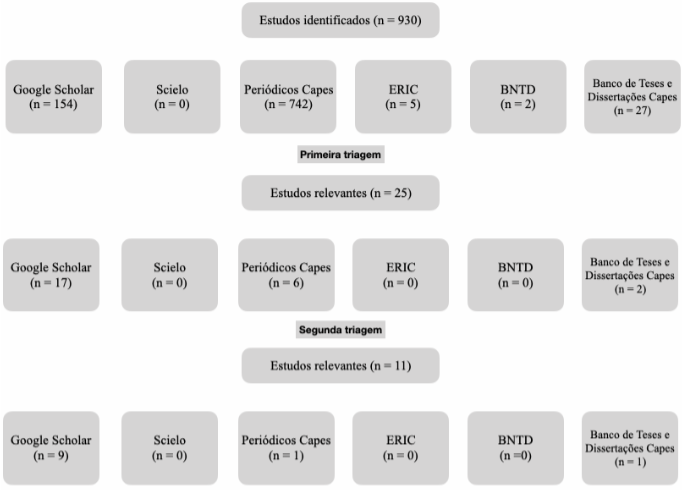
\includegraphics[width=0.9\textwidth]{fig1.png}
 \caption{Esquema da busca de dados nas bases}
 \label{fig1}
 \source{Elaborado pela própria autora (2019)}
\end{figure}

Das onze pesquisas incluídas nessa revisão, 6 são dissertações de mestrado, 3 são trabalhos de conclusão de curso de graduação, e apenas 2 são artigos científicos. A base de dados com mais pesquisas incluídas foi o Google Scholar com nove trabalhos considerados, seguida do Periódico da Capes e do Banco de Teses e Dissertações da Capes, ambos com apenas um trabalho incluído. Algumas bases como a Scielo, ERIC e BNTD não tiveram nenhum trabalho significativo para a presente revisão (\Cref{fig2}). 

\begin{figure}[htbp]
 \centering
 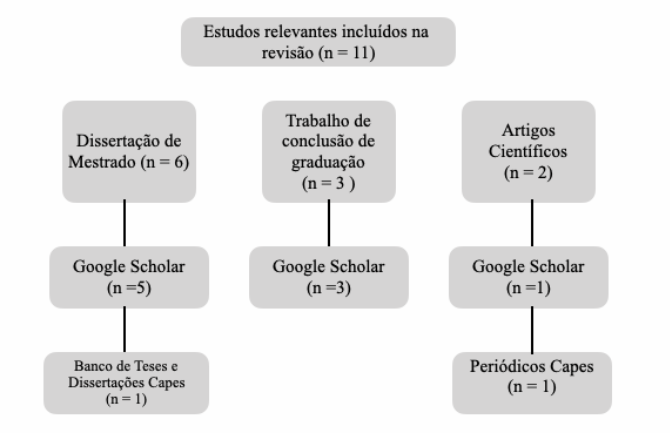
\includegraphics[width=0.75\textwidth]{fig2.png}
 \caption{Base de dados e tipos de trabalhos encontrados}
 \label{fig2}
 \source{Elaborado pela própria autora (2019)}
\end{figure}

\subsection*{Quanto à busca na base de dados: Anos das publicações}
Como observado no gráfico da \Cref{fig3}, é possível notar que a maior parte dos trabalhos incluídos nesta revisão foram publicados no período de 2014 a 2018, havendo uma maior concentração no ano de 2017, com 5 trabalhos publicados nesse período. 

\begin{figure}[htbp]
 \centering
 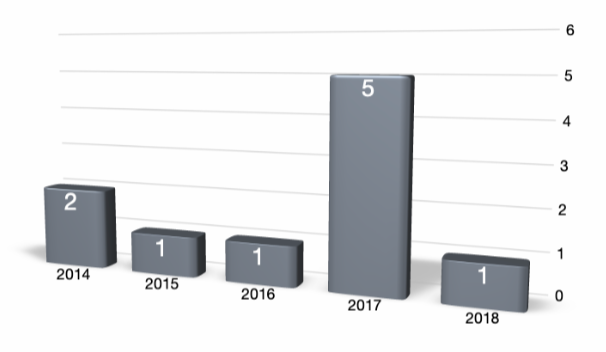
\includegraphics[width=0.7\textwidth]{fig3.png}
 \caption{Número das pesquisas incluídas na revisão distribuídas por anos}
 \label{fig3}
 \source{Elaborado pela própria autora (2019)}
\end{figure}

\subsection*{Quanto à busca na base de dados: Países de origem das publicações}
A maioria dos trabalhos têm origem brasileira, fato já imaginado, pois metade das bases de dados utilizadas eram voltadas à produção científica do Brasil (BNTD, Periódicos da Capes e Banco de teses e dissertações da Capes), bases importantes para pesquisar o estado da arte no país da referente pesquisa, sendo 5 trabalhos do total de 11 de origem brasileira (\Cref{fig4}). 

\begin{figure}[htbp]
 \centering
 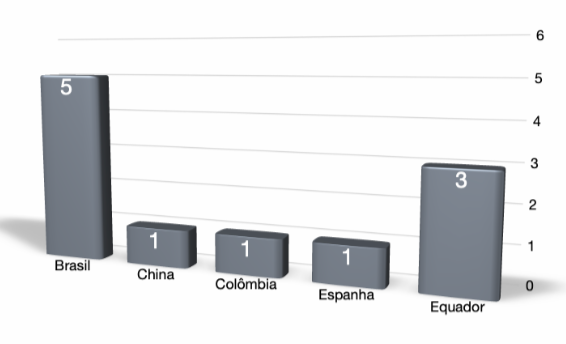
\includegraphics[width=0.7\textwidth]{fig4.png}
 \caption{Número de estudos incluídos por país}
 \label{fig4}
 \source{Elaborado pela própria autora (2019)}
\end{figure}

Com relação aos trabalhos desenvolvidos no Brasil, a \Cref{tab4} traz a especificação de cada universidade e cidades nas quais as pesquisas foram feitas.

\begin{table}[htpb]
\caption{Pesquisas brasileiras distribuídas quanto às universidades e cidades de realização}
\label{tab4}
\centering
\begin{tabular}{ll}
\toprule 
Universidade & Cidade
\\
\midrule
Universidade do Estado da Bahia	& Feira de Santana
\\
Universidade Federal da Paraíba	& João Pessoa
\\
Universidade Federal do Federal do Maranhão	& Codó
\\
Universidade Federal Rural de Pernambuco & Recife
\\
Universidade Tecnológica Federal do Paraná & Londrina
\\ 
\bottomrule
\end{tabular}
\source{Elaborado pela própria autora (2019)}
\centering
\end{table}

Dessa forma, nota-se que a preocupação em estudar e pesquisar sobre os aplicativos como recurso didático no ensino formal de língua estrangeira é prioritariamente mais desenvolvido na região nordeste, contando com 4 trabalhos. A região sul apresenta apenas 1 trabalho, e as outras regiões não apresentam registros. 

\subsection{(Q2) Quais os níveis de escolaridade contemplados pela utilização dos aplicativos móveis como recurso didático?}
Esta revisão enfoca no uso dos aplicativos móveis na rede básica de ensino, ou seja, ensino fundamental e médio, sendo este um dos critérios de seleção. Apenas um dos estudos encontrados \cite{almeida2018} não especificou qual a etapa escolar (fundamental ou médio), mas informou que foi em uma escola de formação básica. Outro estudo apontou que foi realizado no ensino fundamental, mas não especificou o ano escolar. Os demais estudos apresentam todas as informações de nível e ano escolar. A \Cref{fig5} aponta os estudos distribuídos por nível de escolaridade. 

\begin{figure}[htbp]
 \centering
 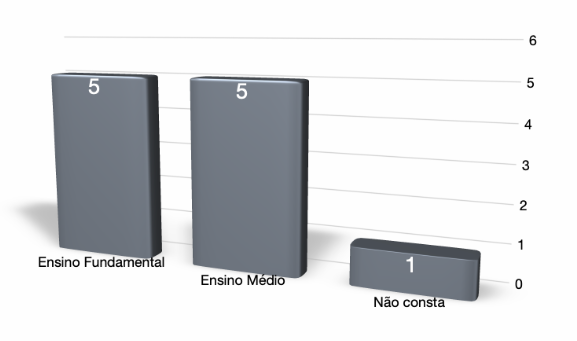
\includegraphics[width=0.7\textwidth]{fig5.png}
 \caption{Número de estudos incluídos através da escolaridade}
 \label{fig5}
 \source{Elaborado pela própria autora (2019)}
\end{figure}

Em resposta à pergunta norteadora (Q2), observou-se que, no total dos 11 trabalhos incluídos nesta revisão, desconsiderando um trabalho que não especifica a escolaridade \cite{almeida2018}, tanto o ensino fundamental \cite{censi2017, nascimento2017, montes2018, ximena2017, lu2014} quanto o ensino médio \cite{rodrigues2014, magali2017, macias2016, redondo2017, liz2015} figuraram em 5 trabalhos com a utilização de aplicativos como recursos didáticos.

\subsection{(Q3) Quais os principais objetivos das pesquisas que utilizaram aplicativos móveis?}
Sobre os objetivos gerais dos estudos selecionados, foram encontrados três eixos centrais nos quais esses trabalhos se encaixam. Um primeiro eixo é ligado ao objetivo de investigar e compreender como os Apps influenciam no ensino-aprendizagem da língua estrangeira ou de alguma habilidade linguística específica. Outro ponto é sobre utilizar os Apps para otimizar, complementar, facilitar, melhorar o processo de ensino-aprendizagem ou o de alguma habilidade linguística. O último objetivo central diz respeito ao desenvolvimento de aplicativos para as aulas de línguas estrangeiras pautados em objetivos linguísticos ou em vertentes teórico-linguísticas. A \Cref{fig6} mostra como os trabalhos estão divididos em números em relação a seus objetivos principais. 

\begin{figure}[htbp]
 \centering
 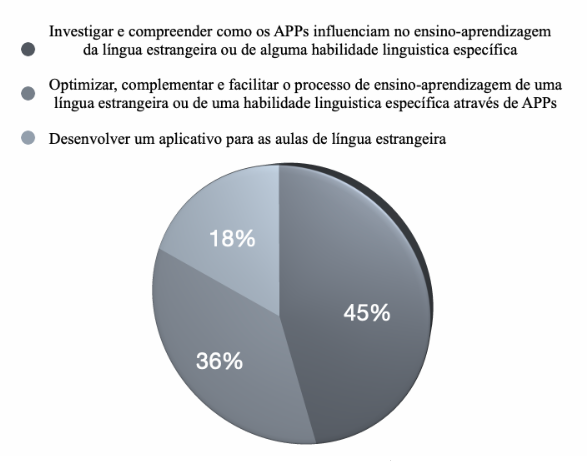
\includegraphics[width=0.7\textwidth]{fig6.png}
 \caption{Números de estudos através de seus objetivos gerais}
 \label{fig6}
 \source{Elaborado pela própria autora (2019)}
\end{figure}

\subsection{(Q4) Qual(is) o(s) objetivo(s) linguísticos para a utilização do(s) APP(s)?}
Quando os aplicativos são usados nas aulas de línguas estrangeiras, é primordial que sejam utilizados para alcançar algum objetivo específico. Sendo assim, a \Cref{fig7} traz os principais objetivos linguísticos quanto ao uso dos aplicativos em sala de aula. Os objetivos perpassam por: investigar e compreender como os Apps influenciam no ensino-aprendizagem de língua estrangeira de alguma habilidade linguística \cite{almeida2018, censi2017, macias2016, magali2017, nascimento2017}; otimizar, complementar e facilitar o ensino-aprendizagem de uma língua estrangeira ou de uma habilidade linguística específica através de Apps \cite{lu2014, montes2018, redondo2017, ximena2017}; e desenvolver um aplicativo para as aulas de língua estrangeira \cite{liz2015, rodrigues2014}.

Vale ressaltar que muitos dos estudos analisados apresentaram mais de um objetivo linguístico, alguns tinham como foco as expressões oral e escrita, outros as quatro habilidades linguísticas, outros vocabulários e as quatro habilidades. Por conta disso, a quantidade de objetivos linguísticos é superior à de trabalhos encontrados. 

\begin{figure}[htbp]
 \centering
 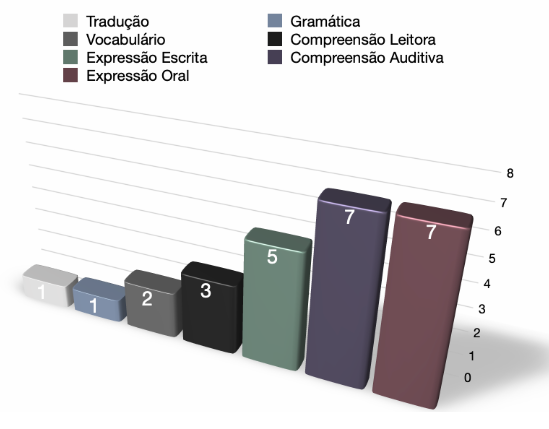
\includegraphics[width=0.7\textwidth]{fig7.png}
 \caption{Objetivos linguísticos dos estudos incluídos}
 \label{fig7}
 \source{Elaborado pela própria autora (2019)}
\end{figure}

\subsection{(Q5) Quais os \textit{Apps} utilizados e quais os conteúdos abordados?}
Os aplicativos utilizados nas pesquisas selecionadas se repetiram algumas vezes, algumas pesquisas utilizaram mais que um aplicativo e outras desenvolveram seu próprio aplicativo. No total, foram utilizados 8 aplicativos já existentes e foram desenvolvidos 4. Na \Cref{fig8} exemplificam-se os aplicativos utilizados, junto à quantidade de vezes em que eles apareceram nos estudos selecionados, pois, como mencionado anteriormente, alguns dos trabalhos utilizaram mais de um \textit{APP} para a sua pesquisa.

\begin{figure}[htbp]
 \centering
 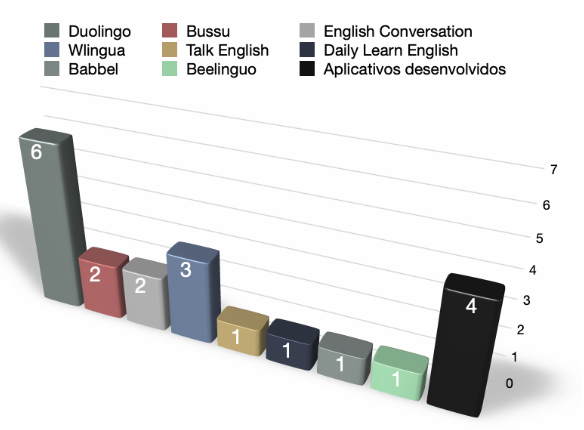
\includegraphics[width=0.7\textwidth]{fig8.png}
 \caption{Aplicativos utilizados nos estudos distribuídos pelo número de utilização}
 \label{fig8}
 \source{Elaborado pela própria autora (2019)}
\end{figure}

Os quatro aplicativos que constam na \Cref{fig8} como "Apps desenvolvidos para a pesquisa" são intitulados de English Gap \cite{rodrigues2014}, Audio Trainer Play \cite{redondo2017}, Learning Chinese \cite{lu2014} e High Fly Learning \cite{liz2015}.

\section{Discussão}
A pergunta principal que esta revisão pretende responder é: "existe a utilização de aplicativos móveis como recurso didático nas aulas de língua estrangeira na educação básica?" Com os dados levantados na presente pesquisa, e considerando-se que pouco se registra do que é desempenhado dentro de sala de aula, ainda assim, foram encontrados alguns trabalhos com essa temática. Entretanto, elas se diferenciam em muitos aspectos, seja nos aplicativos utilizados, na escolaridade aplicada ou nos objetivos de implementação do recurso digital.

O número total de 11 trabalhos selecionados \cite{censi2017, nascimento2017, montes2018, ximena2017, lu2014, rodrigues2014, magali2017, macias2016, redondo2017, liz2015}, dentre 930 encontrados nas buscas, mostra que dentro da questão do uso dos aplicativos para língua estrangeira apenas esse pequeno número é efetivamente utilizado e registrado em sala de aula para fins pedagógicos na educação básica. Por se tratar de uma prática, muito do que é feito não é registrado e nem publicado com carácter de pesquisa, explicando este baixo número de trabalhos encontrados. Por conta dos critérios de exclusão e inclusão, ficaram de fora os trabalhos com a utilização de \textit{Apps} em curso superior ou com educação não-formal. Sendo assim, ainda se nota a necessidade de mais estudos voltados para o uso das tecnologias digitais para o ensino de línguas estrangeiras na educação básica. Para \textcite{saccol2011} essa tecnologia é muito promissora, pois permite baixo custo, rápida difusão de informações, interação entre pessoas e sistemas, além de viabilizar novas abordagens pedagógicas.
	
Sobre a distribuição dos números de pesquisas brasileiras, é curioso e contraditório estarem concentrados na região nordeste, pois, de acordo com o \textcite{cetic2017}, o Nordeste apresenta apenas 30\% das suas instituições públicas de ensino com conexão à internet, mas, ao mesmo tempo, é a região na qual os alunos mais acessam a internet via celular nas escolas (29\%), sendo que nas outras regiões, como a Sul e a Sudeste, o percentual de uso é de com 10\% e 14\%, respectivamente \cite{cetic2017}. Esses percentuais podem ser resultado também de políticas públicas, municipais ou estaduais que restringem o uso de celular em sala de aula. Esses dados também apontam a falta de infraestrutura das escolas na região Nordeste, o que faz com que o celular pessoal se torne uma alternativa viável quando muitas vezes a escola não dispõe dos aparatos tecnológicos de maneira satisfatória, como computadores com acesso à internet.

Em relação ao nível de escolaridade referente à utilização de aplicativos móveis como recurso didático nas aulas de língua estrangeira, não se pode relatar nenhum perfil, pois os números encontrados no ensino fundamental e no ensino médio foram homogêneos, não houve destaque para uma etapa em específico. 

Quanto aos objetivos dos estudos, o resultado mais recorrente de 45\% deles foi de investigar e compreender como os \textit{Apps} influenciam no ensino-aprendizagem da língua estrangeira ou de alguma competência linguística específica. Nota-se que existem essas preocupações em saber de que forma as tecnologias digitais podem afetar o ensino de LE dentro de sala de aula, se efetivamente podem potencializar o processo de ensino-aprendizagem e se realmente podem ser utilizadas como um recurso didático eficaz. 

O segundo objetivo com a maior porcentagem, de 36\%, é o de otimizar, complementar e facilitar o processo de ensino-aprendizagem de uma língua estrangeira ou de uma competência linguística específica através de \textit{Apps}. Isso já demonstra que de alguma maneira a utilização de aplicativos em sala de aula positivamente, e também, traz um olhar mais objetivo e prático na instauração desse recurso, afirmando que de alguma forma irá potencializar alguma etapa do processo. 

Quando o objetivo é o desenvolvimento desse recurso didático o número já diminui, demonstrando que o desenvolvimento de recursos didáticos digitais por parte dos professores-pesquisadores não é uma de suas prioridades. Sobre esses aplicativos que foram desenvolvidos recaem fatores similares, já que nenhum dos dois utiliza as potencialidades que um aplicativo pode oferecer, e na maioria das vezes, são atividades que podemos desenvolver em um livro didático, mas transpostas para a tela do celular através de um aplicativo móvel. Percebeu-se uma grande ocorrência no número de atividades de expressão escritas e de preenchimento de lacunas (\Cref{fig9} e \ref{fig10}), por mais que os aplicativos dissessem que estavam voltados para a competência comunicativa, para as quatro habilidades. 

\begin{figure}[htbp]
\begin{minipage}[t]{0.35\textwidth}
 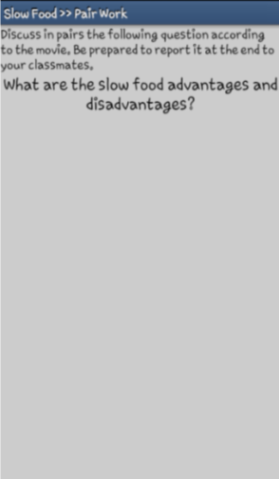
\includegraphics[width=\linewidth]{fig9.png}
 \subcaption{App High Fly Learning.}
 \label{fig9}
\end{minipage}
\hfill
\begin{minipage}[t]{0.35\textwidth}
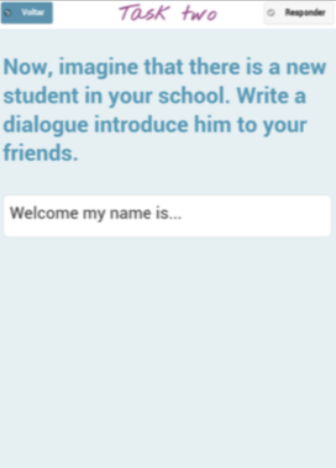
\includegraphics[width=\linewidth]{fig10.png}
\subcaption{App English GAP.}
\label{fig10}
\end{minipage}
\caption{Tela dos aplicativos.}
\label{fig9e10}
\source{Elaborado pela própria autora (2019).}
\end{figure}



As competências voltadas à oralidade (compreensão auditiva e expressão oral) foram os objetivos linguísticos mais buscados, visto que a convergência digital \cite{jenkins2008} facilita o acesso e a utilização de materiais com reprodução de áudio, acabando com a necessidade de o professor trazer à sala de aula os aparatos que antes eram utilizados para esse objetivo, como o rádio e a TV, facilitando o trabalho dos atores envolvidos nos processos de ensino-aprendizagem. 

Há a ocorrência de duas pesquisas que desenvolveram aplicativos, entretanto, isso não constam nos objetivos específicos, pois seus objetivos principais não eram a criação e o desenvolvimento efetivo desses \textit{Apps}, os objetivos se pautavam em aprimorar alguma competência ou habilidade a partir desses aplicativos previamente elaborados. Sendo assim, respondendo à pergunta sobre os aplicativos utilizados, dentre os que apareceram na busca, apenas quatro foram desenvolvidos pelos próprios autores \cite{rodrigues2014, liz2015, redondo2017, lu2014}; porém, quando perguntados sobre os seus objetivos principais, apenas dois \cite{rodrigues2014, liz2015} tiveram o desenvolvimento como objetivo principal.
	
Entre os aplicativos utilizados nas pesquisas, o que teve mais ocorrências de utilização foi o Duolingo. Esse é o \textit{App} mais baixado e popular entre os de línguas estrangeiras, com mais de 70 milhões de acessos \cite{hickey2015}, o que faz com que ele apareça em primeiro lugar na área de aplicativos educacionais ou quando buscamos um aplicativo com objetivo de aprender língua estrangeira. Esses pontos podem explicar o grande número de utilização do Duolingo frente aos outros \textit{Apps} nesta pesquisa.

Considerando as 17 utilizações referentes a aplicativos já existentes, outros 4 trabalhos \cite{rodrigues2014, liz2015, redondo2017, lu2014} utilizaram e desenvolveram aplicativos para servir como um recurso digital para as aulas de línguas estrangeira no ensino básico. Esse número mostra que os aplicativos que já existem são mais facilmente encontrados e muito mais utilizados, imagina-se que por sua praticidade. Desenvolver um aplicativo, por mais que possa se adequar exatamente às necessidades do professor, implica nas questões que a maioria dos docentes não têm tempo nem formação suficiente para planejá-lo ou desenvolvê-lo. Entretanto, esse pequeno número de trabalhos encontrados também demonstra que há mais pesquisas a serem desenvolvidas sobre aplicativos móveis com o objetivo de serem utilizados como recurso didático digital em sala de aula.

Ainda existem espaços e possibilidades a serem explorados e pesquisados no que diz respeito ao uso de aplicativos móveis como recursos didáticos, visto que há ainda uma escassez de estudos sobre a temática, já que são questões emergentes e atuais. Também, há a necessidade de que se registre e publique mais, pois muito do que se aplica e se pratica em sala de aula não chega a ser registrado em forma de trabalhos científicos, ficando muito restrito à prática. É importante levar em consideração o que diz \textcite{schon2000}, que afirma que o professor deve refletir sobre a sua prática, deve ser um professor pesquisador. Também, por ser uma prática muito recente, e ainda não totalmente conhecida e utilizada por muitos professores-pesquisadores, observa-se certa carência de pesquisas, de metodologias e de práticas pedagógicas nesse âmbito \cite{saccol2011}. 

\section{Conclusão}
Com a evolução das tecnologias digitais, a sociedade se adaptou e se apropriou delas, incorporando-as em muitas atividades cotidianas, principalmente o \emph{smartphone}, que se converteu na extensão de nossas mãos. Por outro lado, quando entramos no ambiente escolar, essa questão e essa mudança parecem ser esquecidas, e as tecnologias digitais são muitas vezes rechaçadas e tachadas como de uso exclusivo para o lazer, que não podem ser incorporadas no processo pedagógico dentro da escola. Entretanto, muitos autores \cite{bannell2016, gardner2014, karsenti2014, perezgomez2012, saccol2011, unesco} já mostraram que as tecnologias móveis podem ser incorporadas como recursos digitais mediadores no processo de ensino-aprendizagem, desde que estejam de acordo com os objetivos pedagógicos, ou seja, desde que o objetivo requisite o uso do recurso, não o contrário. 

No que diz respeito ao uso de aplicativos móveis nas aulas de língua estrangeira da educação básica, esta revisão sistemática demonstrou que o uso é ainda pouco registrado, e quando há utilização, na maioria das vezes, é a partir de aplicativos já disponíveis nas plataformas de \emph{download}. A criação de aplicativos como uma forma de recurso didático é ainda muito escassa por conta de questões que vão desde infraestrutura escolar até formação de professores.  Ainda, muito do que é criado tendo como objetivo a prática pedagógica é pouco registrado, justificando a pequena quantidade encontrada de pesquisas práticas desenvolvidas dentro da sala de aula.

Sobre o desenvolvimento de aplicativos como recursos didáticos nas aulas de línguas estrangeiras no ensino básico, há muito o que explorar quanto às suas potencialidades. Pode-se pensar em apresentar diferentes tipos de atividades utilizando as características que os aplicativos apresentam quanto à questão de ubiquidade e à questão midiática, para que o processo de aprendizagem seja efetivamente potencializado, e não seja apenas uma transposição do papel para a tela do celular. 



\printbibliography\label{sec-bib}
% if the text is not in Portuguese, it might be necessary to use the code below instead to print the correct ABNT abbreviations [s.n.], [s.l.] 
%\begin{portuguese}
%\printbibliography[title={Bibliography}]
%\end{portuguese}


\end{document}
